\section*{Hard Tasks}
Our tool allows to show certain objects attributed with
geographic positions, like buildings, parks, waters, districts, and
photos taken in Berlin.
The user can click on each pair of those objects to get information about
relationships between them.
The tool takes the type of object into account and displays, according
to feasibility, the minimal distance between the objects, whether they lie
inside of each other, and how the objects intersect following the 9-cut model.

The photos from the website Flickr are all tagged as Brandenburg gate.
Therefore, we show them as points with a size proportional to
the distance to the landmark.
Hovering over a photo displays the picture next to the mouse
as seen in \figref{brandenburg}.

\begin{figure}[b]
\centering
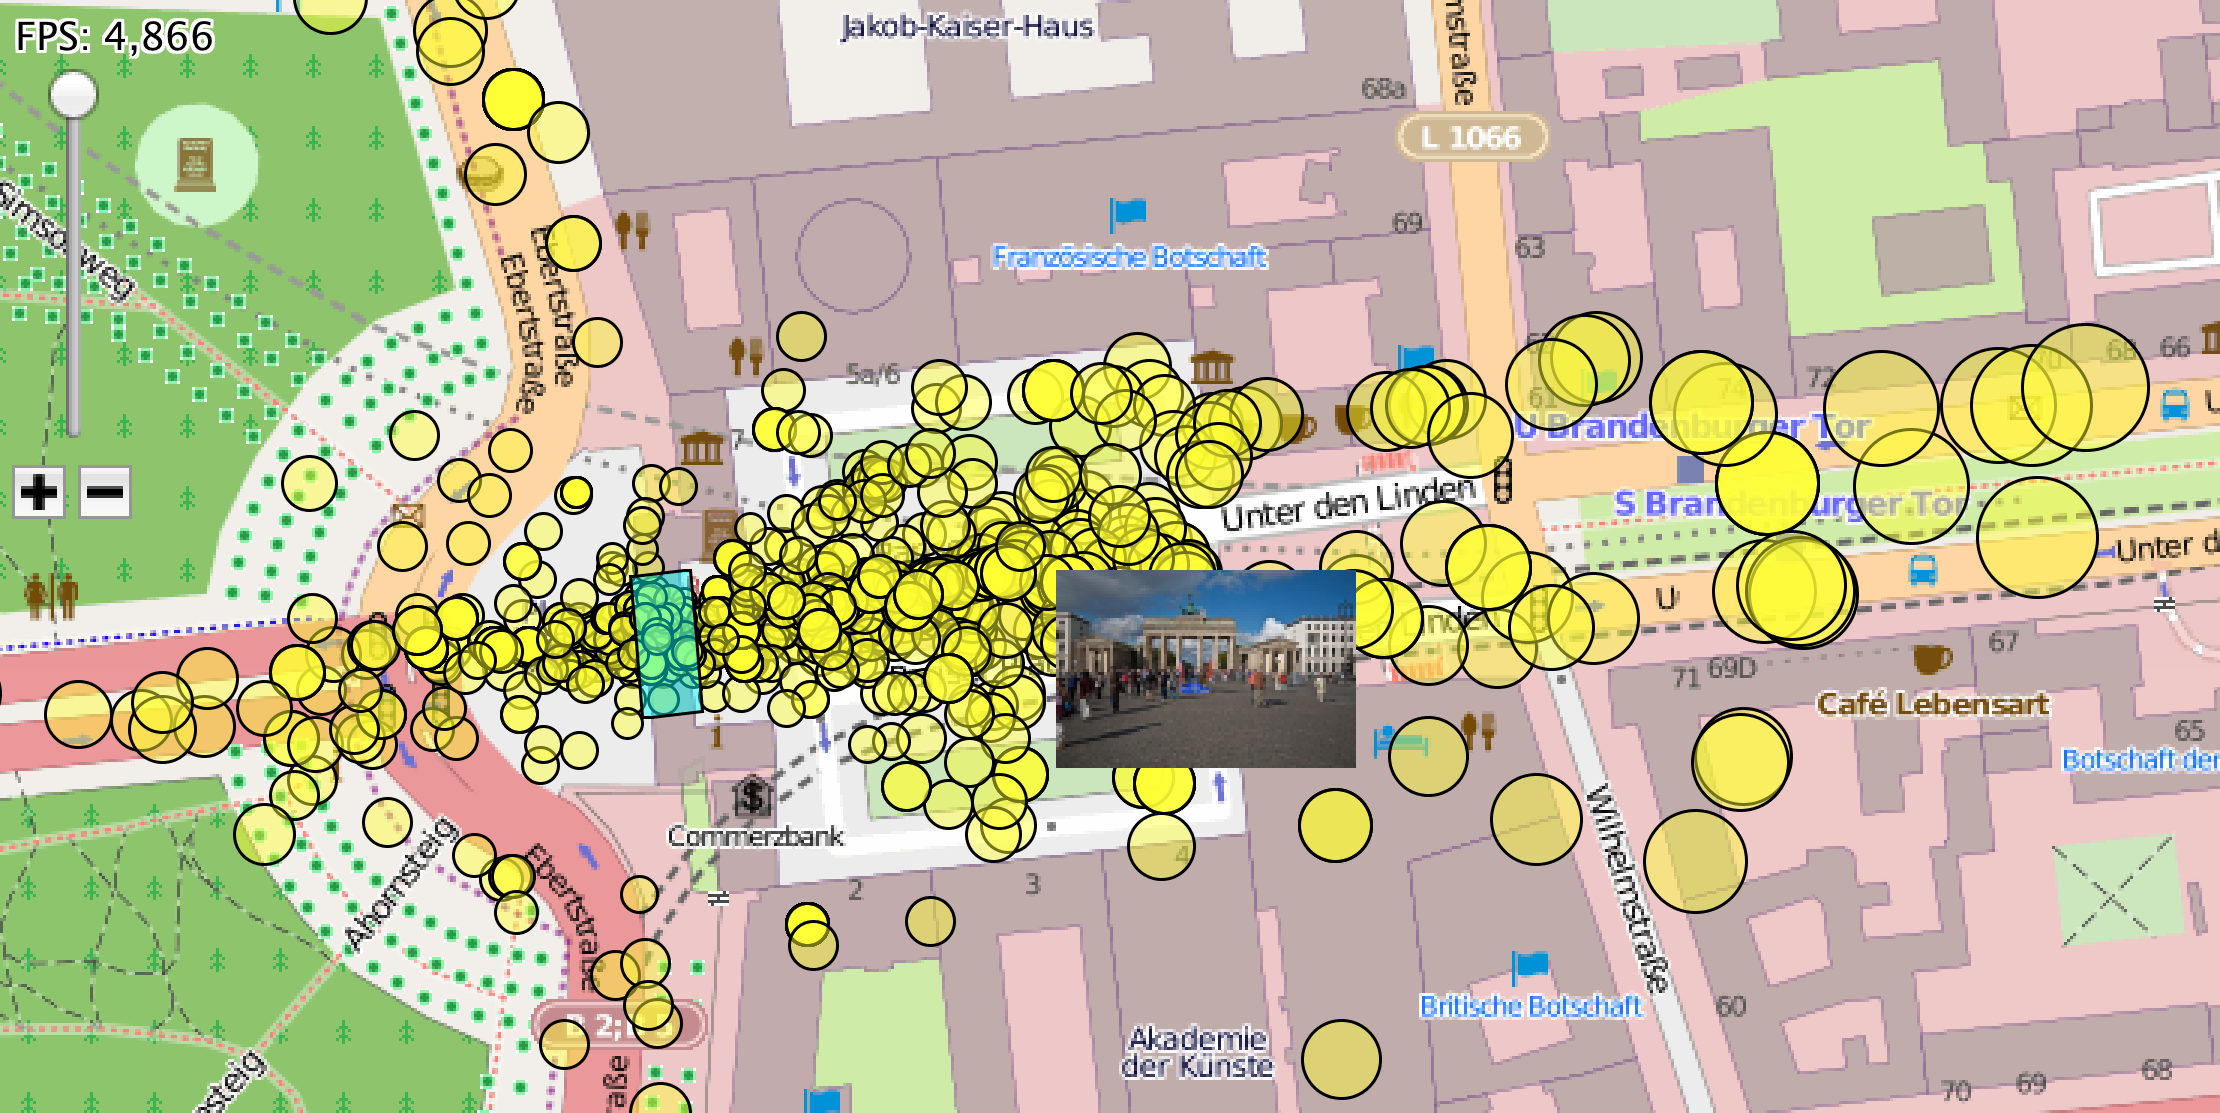
\includegraphics[width=0.9\linewidth]{imgs/brand}
\caption{Photos tagged as Brandenburg gate. The size of the dots
is proportional to the distance to the actual landmark.
A hovered photo shows the actual picture.}
\label{fig:brandenburg}
\end{figure}

Choropleth maps show the ratio of the areas of commercial buildings to their surrounding
district (\figref{commercial}) and the relative amount of
Flickr photos in a district (\figref{flickr}).
\figref{parks} shows parks and whether they are near water.
\begin{figure}
        \centering
		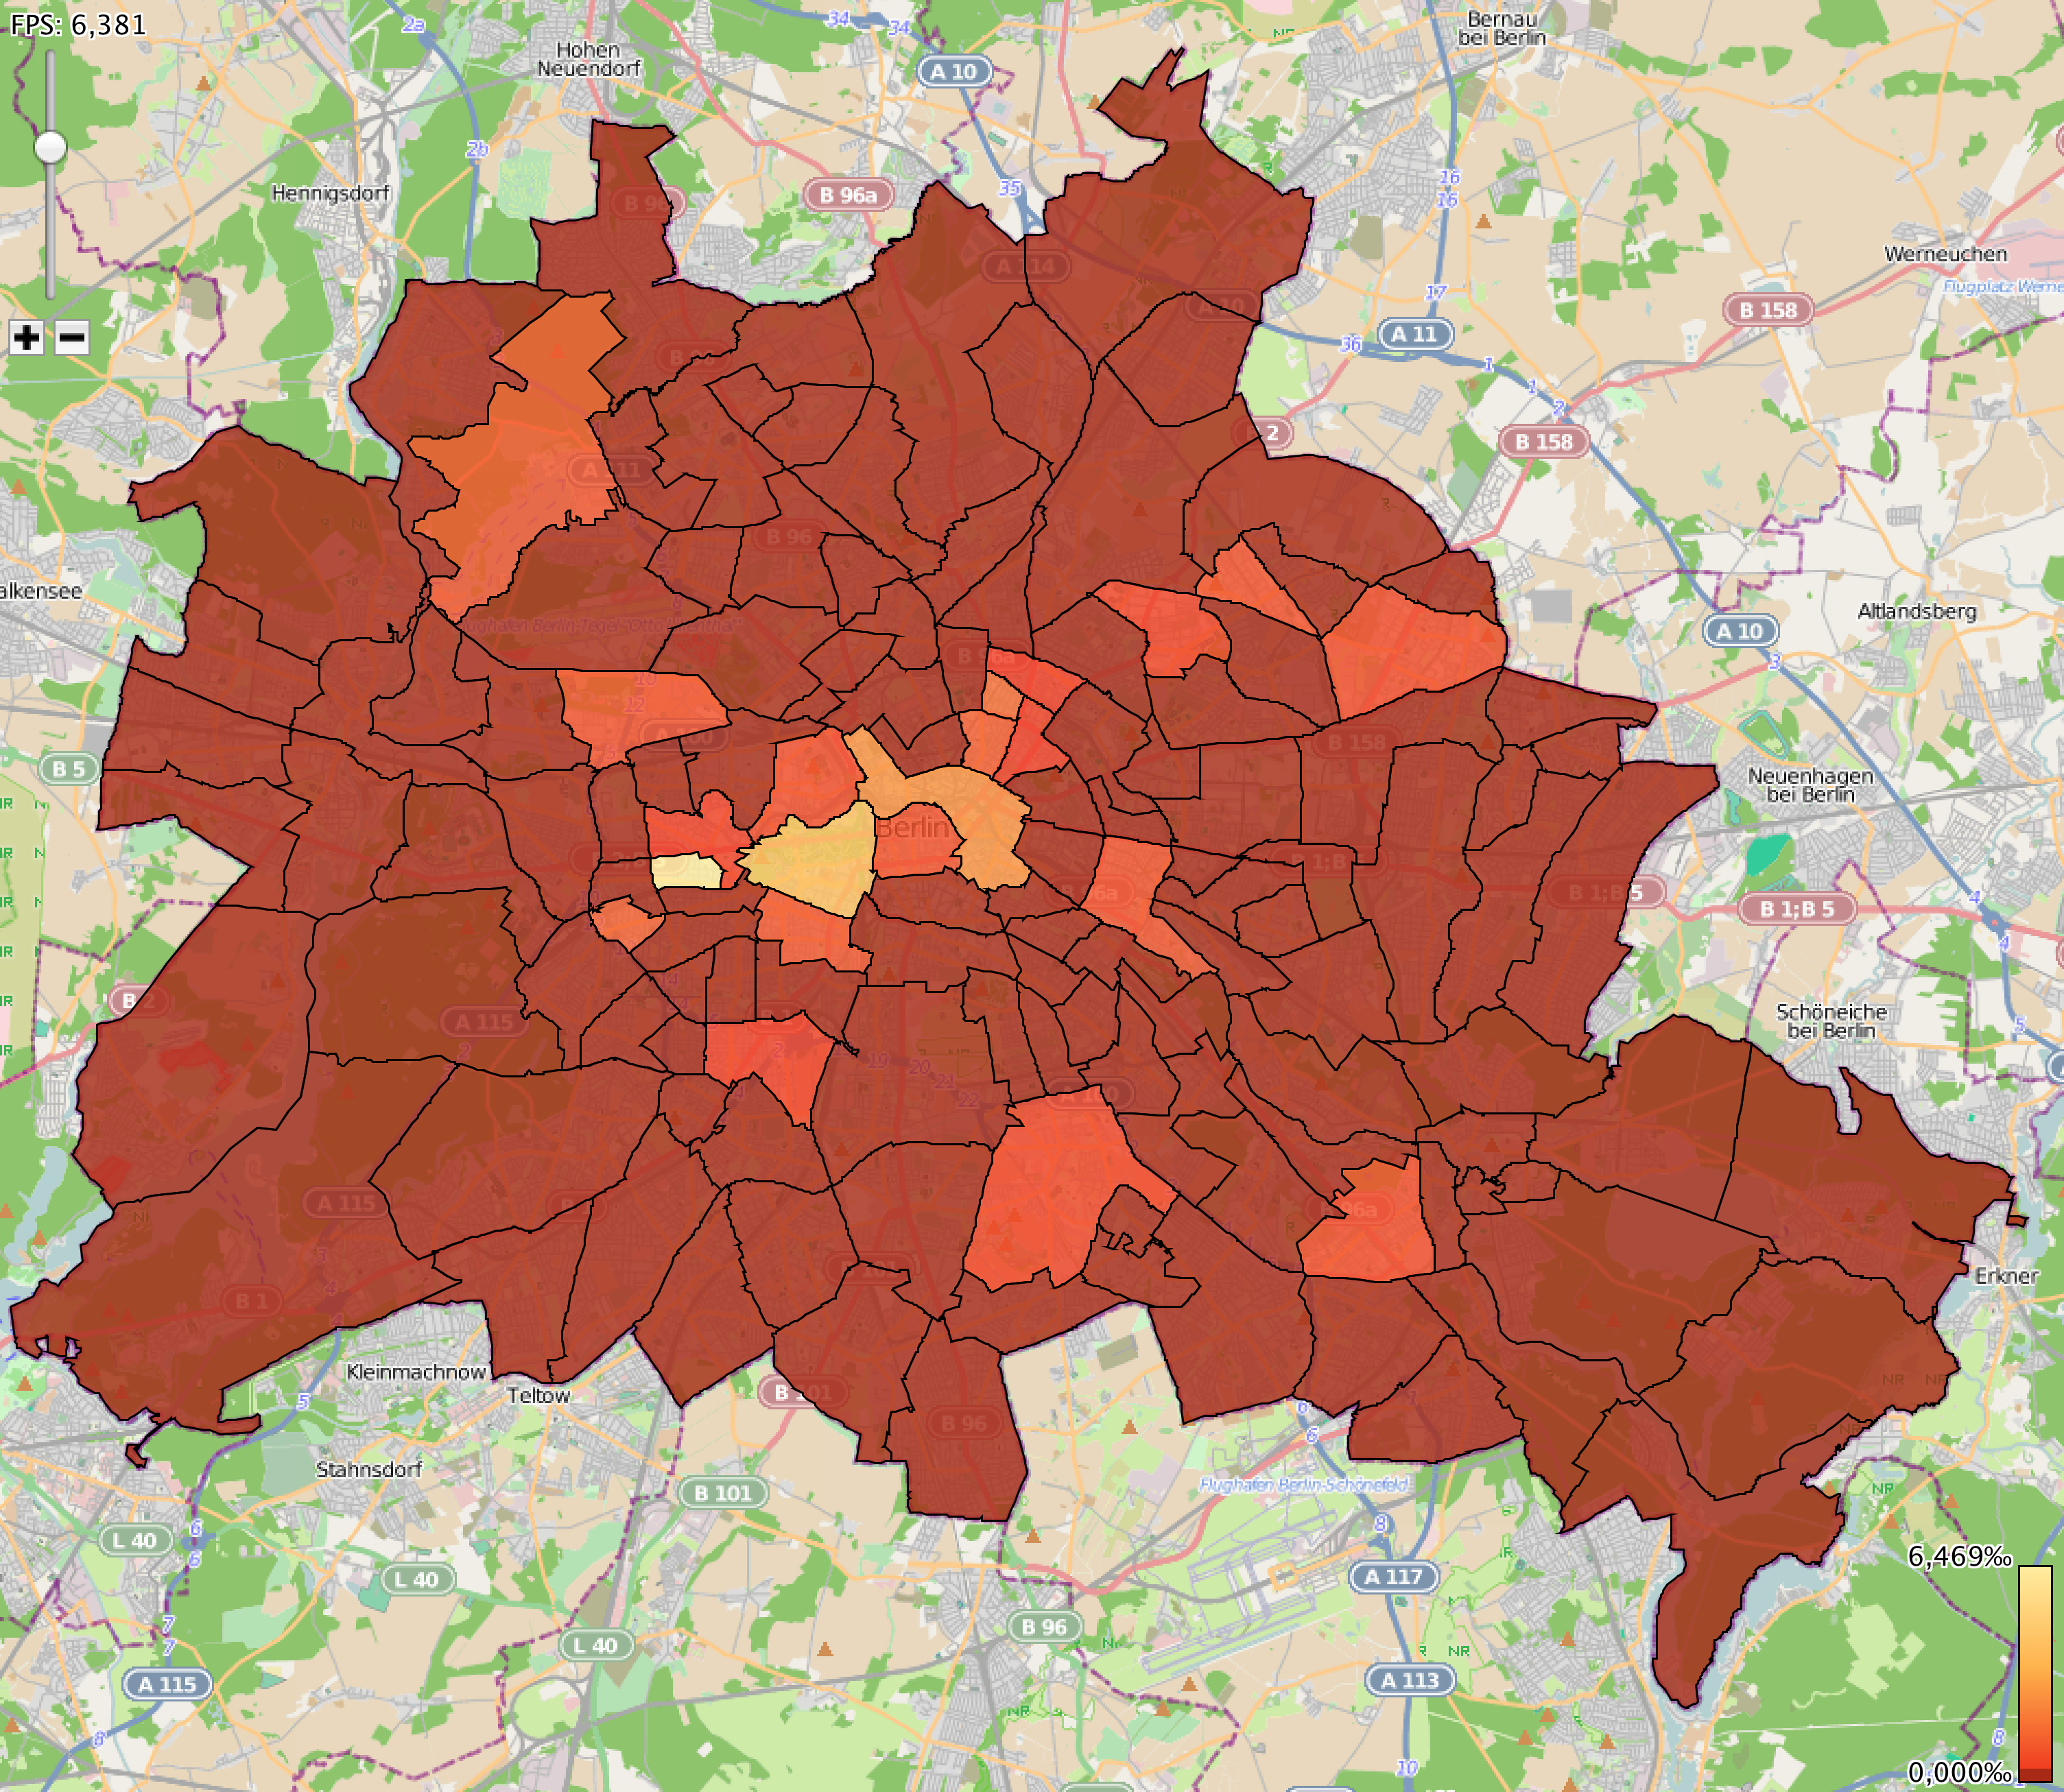
\includegraphics[width=0.6\linewidth]{imgs/commercial}
        \caption{A choropleth map showing the ratio of the area of commercial buildings
        per district to the area of the district.}
		\label{fig:commercial}
\end{figure}
An overlay (\figref{museum}) shows distances to the nearest museum mapped as color.
We modified the standard scan-line approach of calculating the distance field to
increase accuracy and reduce visual artifacts while maintaining computation time.
This is done by storing a reference to the closest target pixel for each visited
pixel and calculating exact distances to them. For more accurate
results, we expanded the area covered by algorithms beyond the view-port.
\begin{figure}[b]
        \centering
		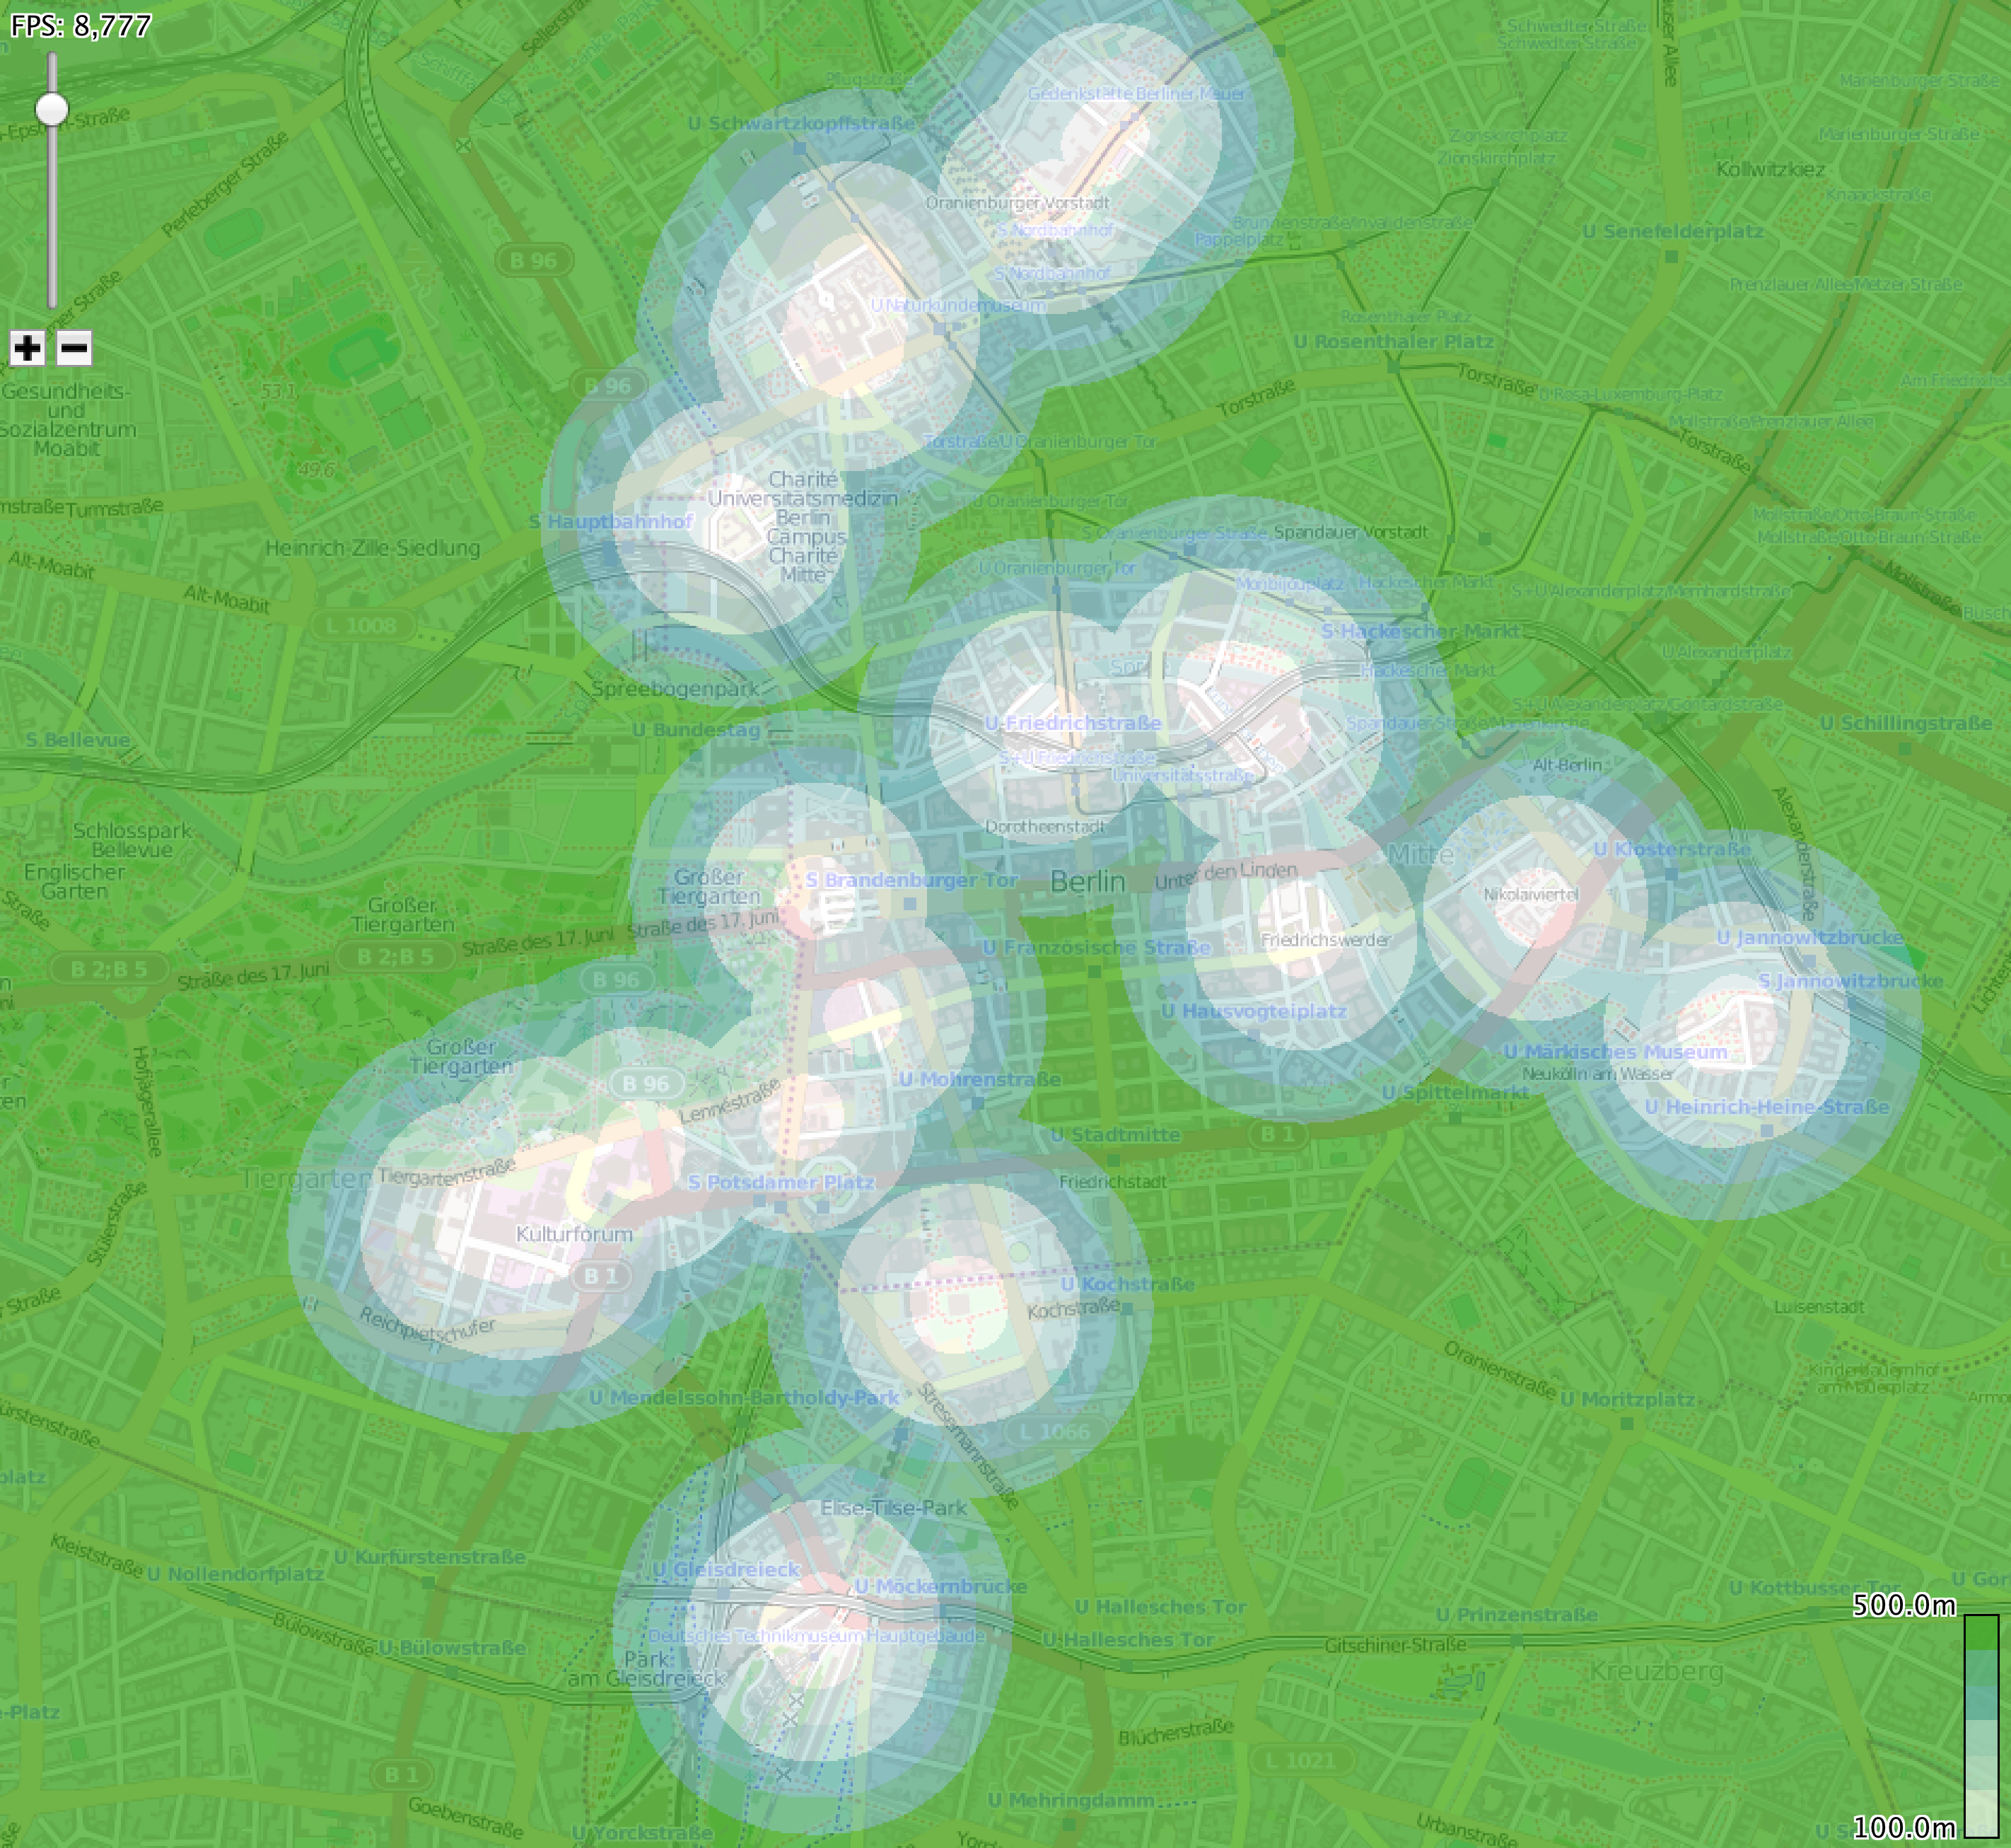
\includegraphics[width=0.4\linewidth]{imgs/museum}
        \caption{Showing distances to nearby museums encoded as color. White regions
        are near to a museum and green areas are further away than $500m$ to the
        nearest museum.}
		\label{fig:museum}
\end{figure}
\begin{figure*}[t]
		\centering
		\begin{subfigure}[b]{0.225\textwidth}
                \centering
                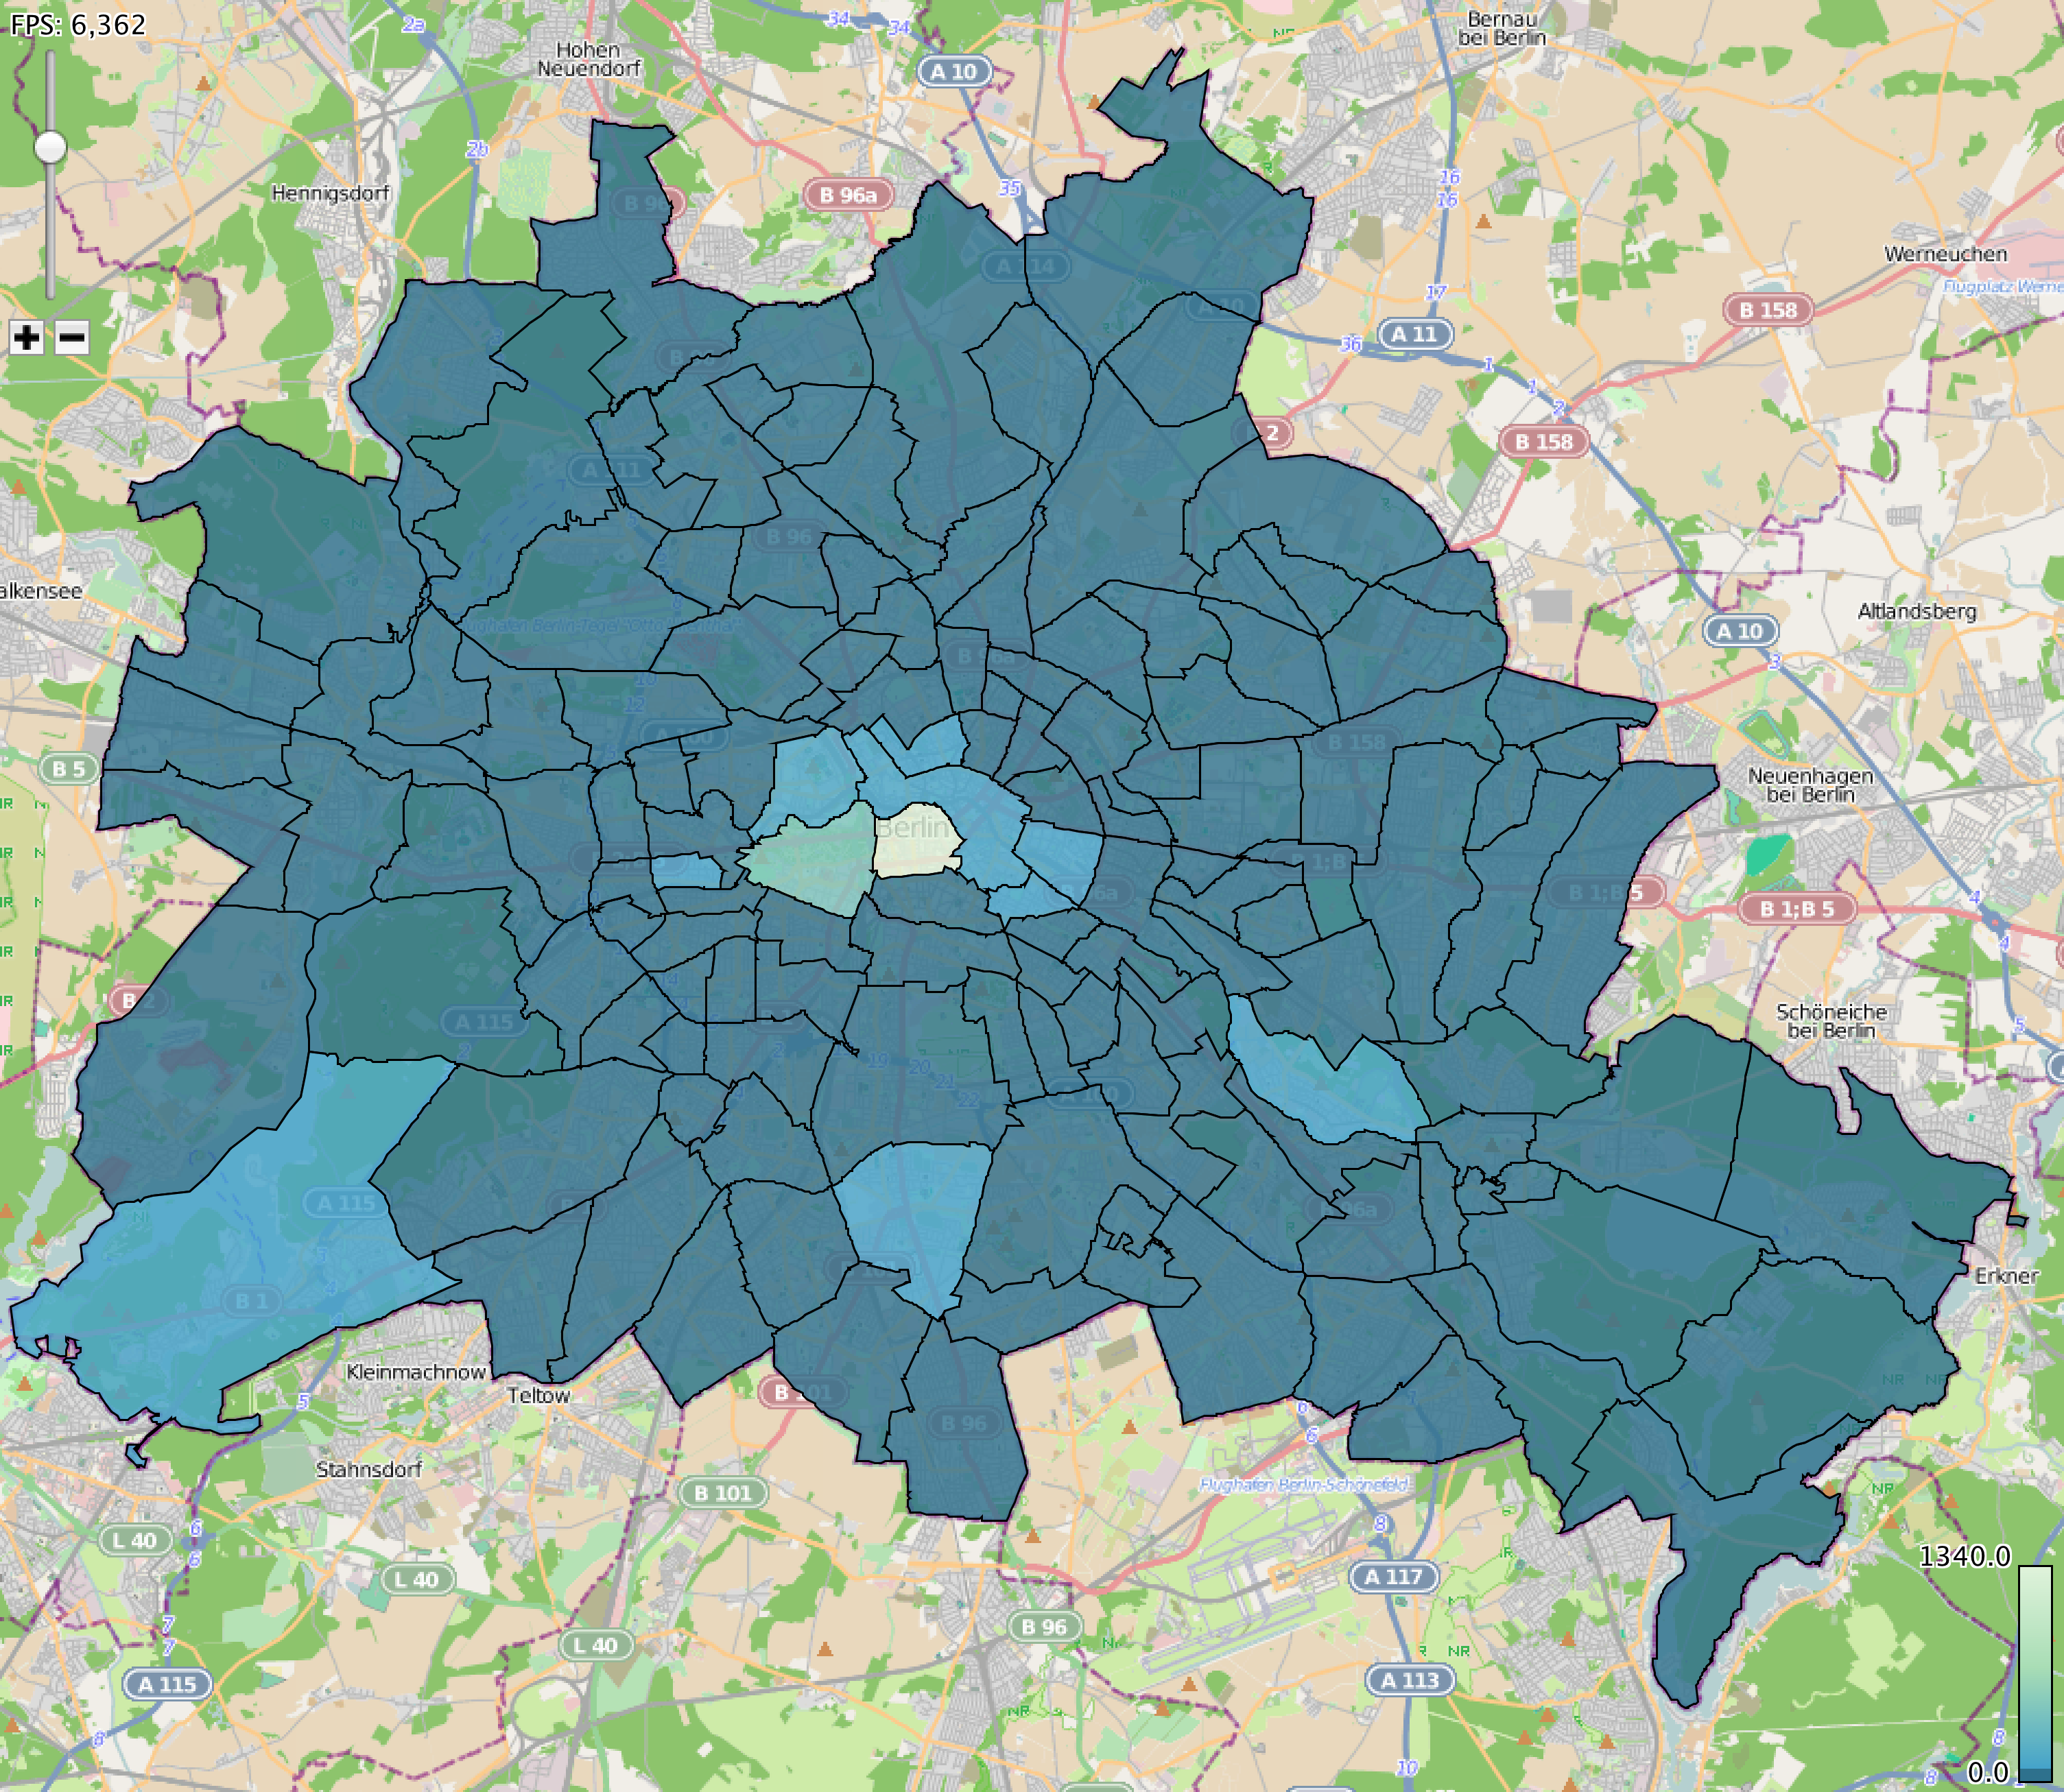
\includegraphics[width=\textwidth]{imgs/flickr}
                \caption{A choropleth map showing the relative amount of flickr photos tagged
                as Brandenburg gate.}
                \label{fig:flickr}
        \end{subfigure}
        \hspace*{0.02\textwidth}
        \begin{subfigure}[b]{0.225\textwidth}
				\centering
				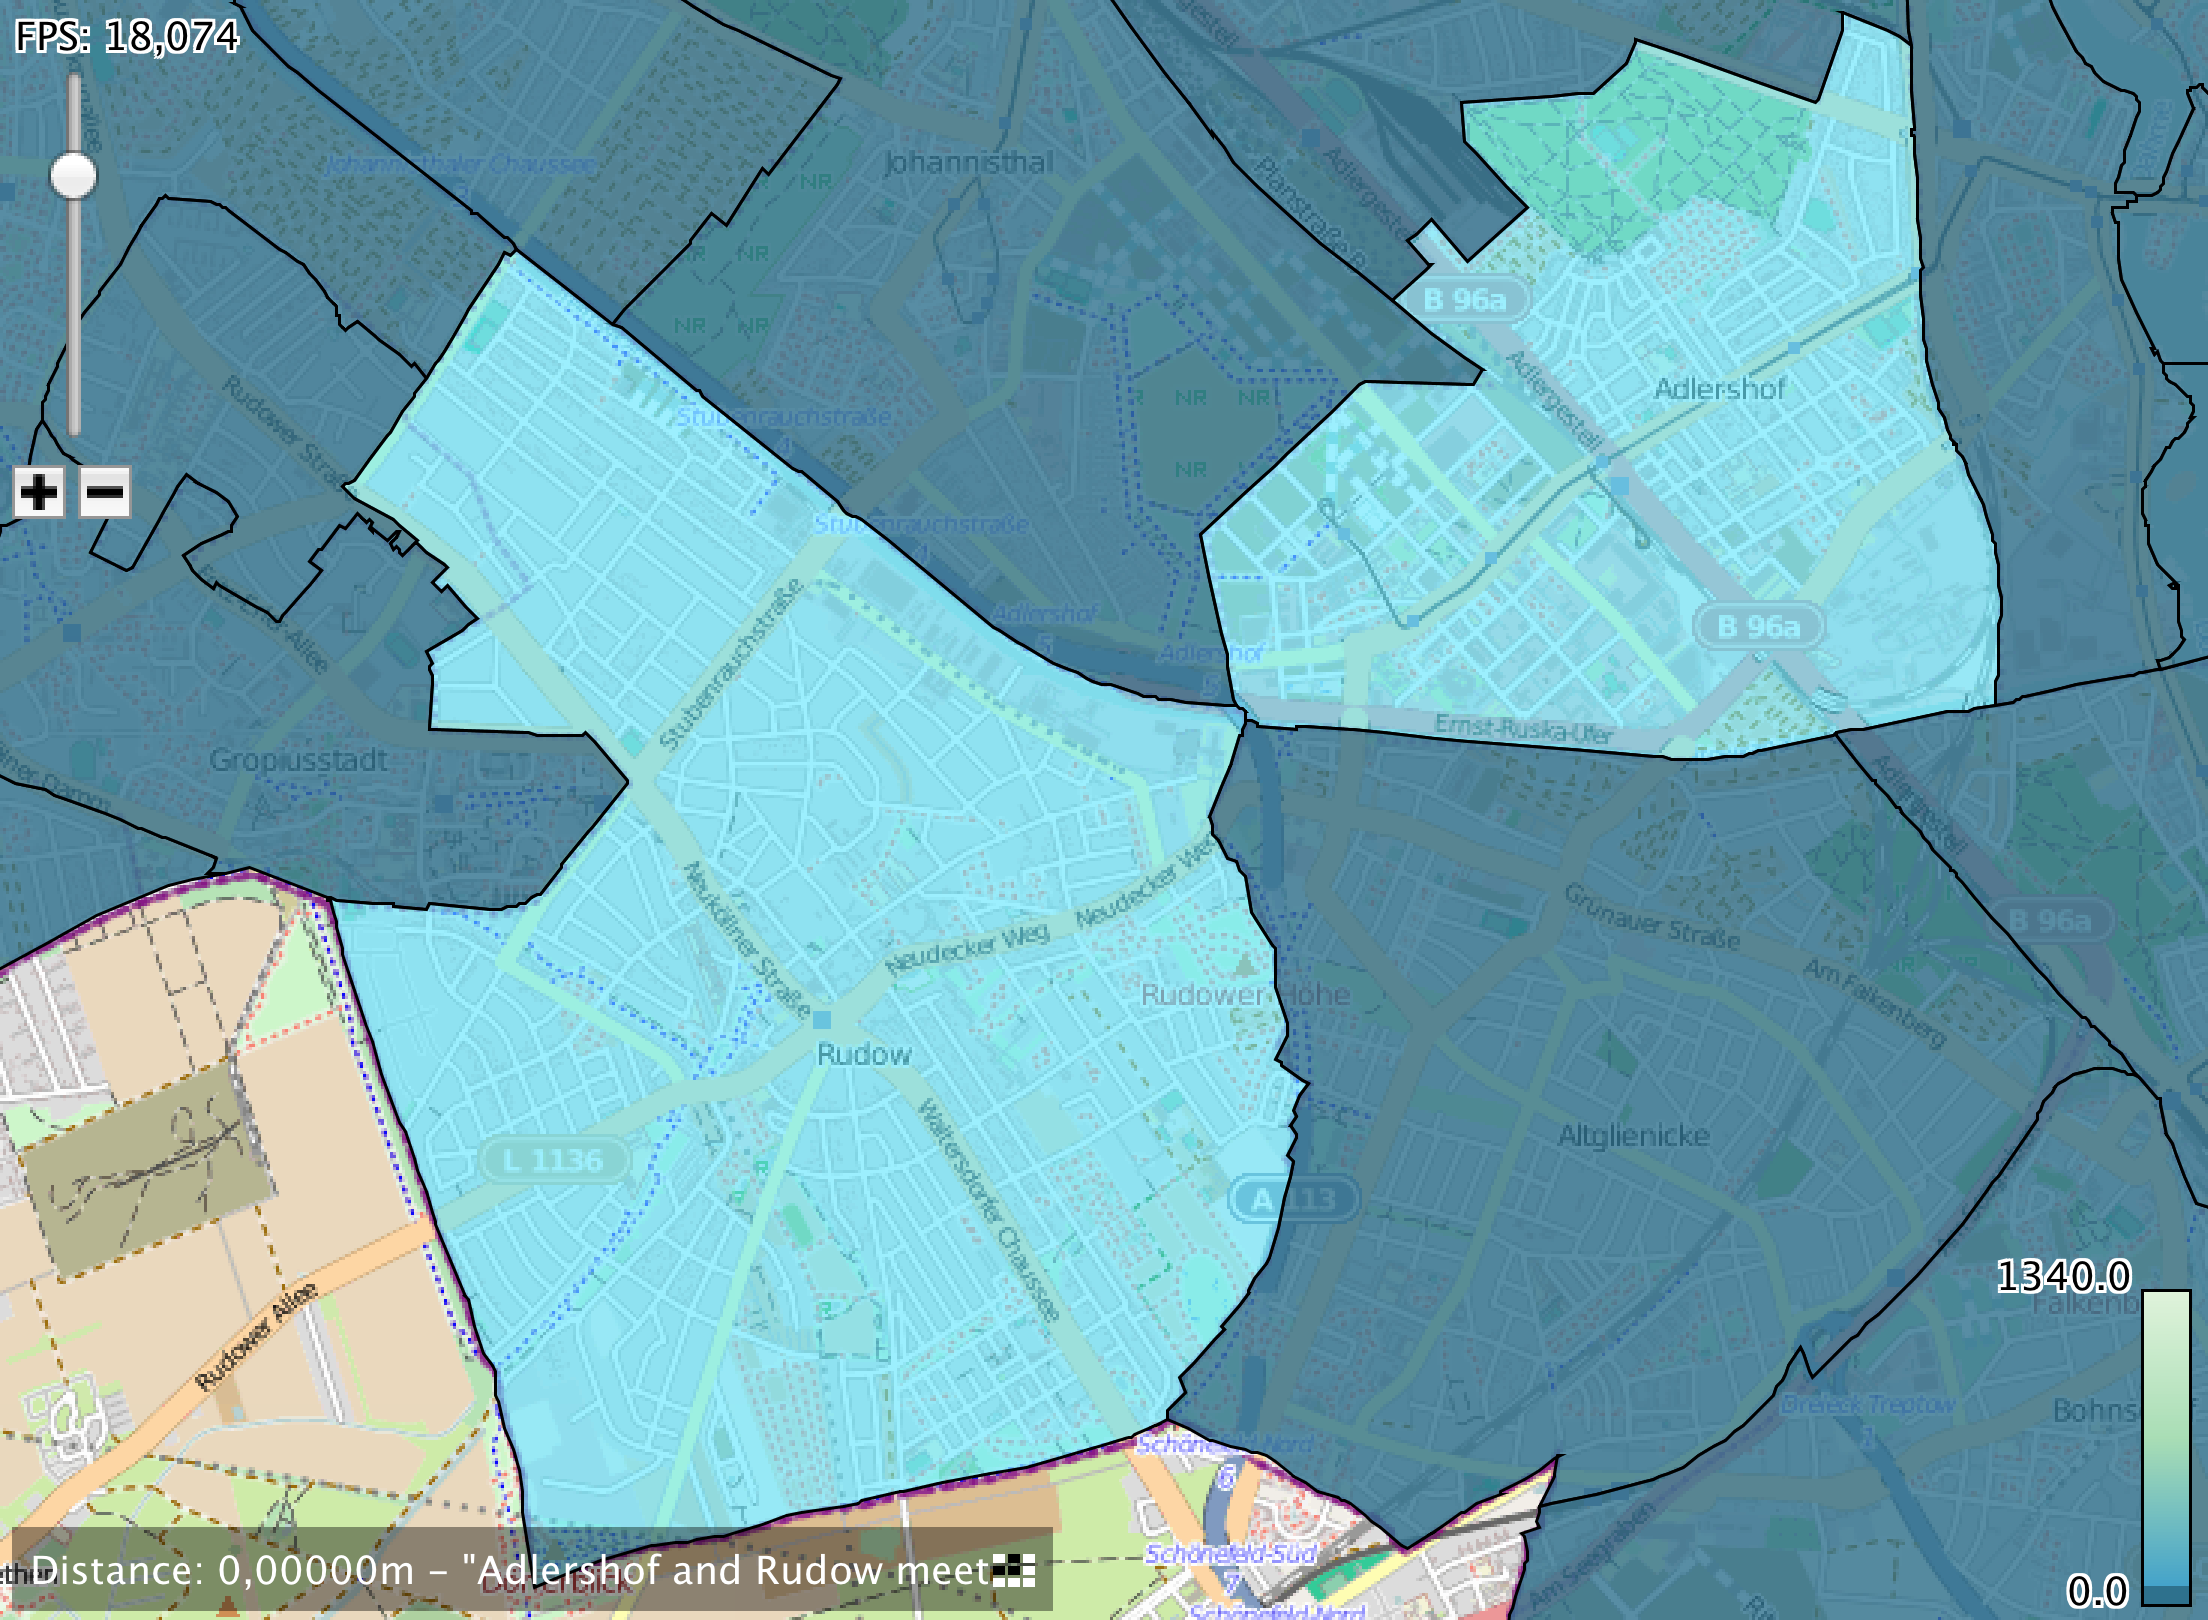
\includegraphics[width=\textwidth]{imgs/rel}
				\caption{A selection of two districts showing the message that
				they meet along with the corresponding 9-cut matrix.}
				\label{fig:rel}
		\end{subfigure}
		\hspace*{0.02\textwidth}
        \begin{subfigure}[b]{0.225\textwidth}
                \centering
                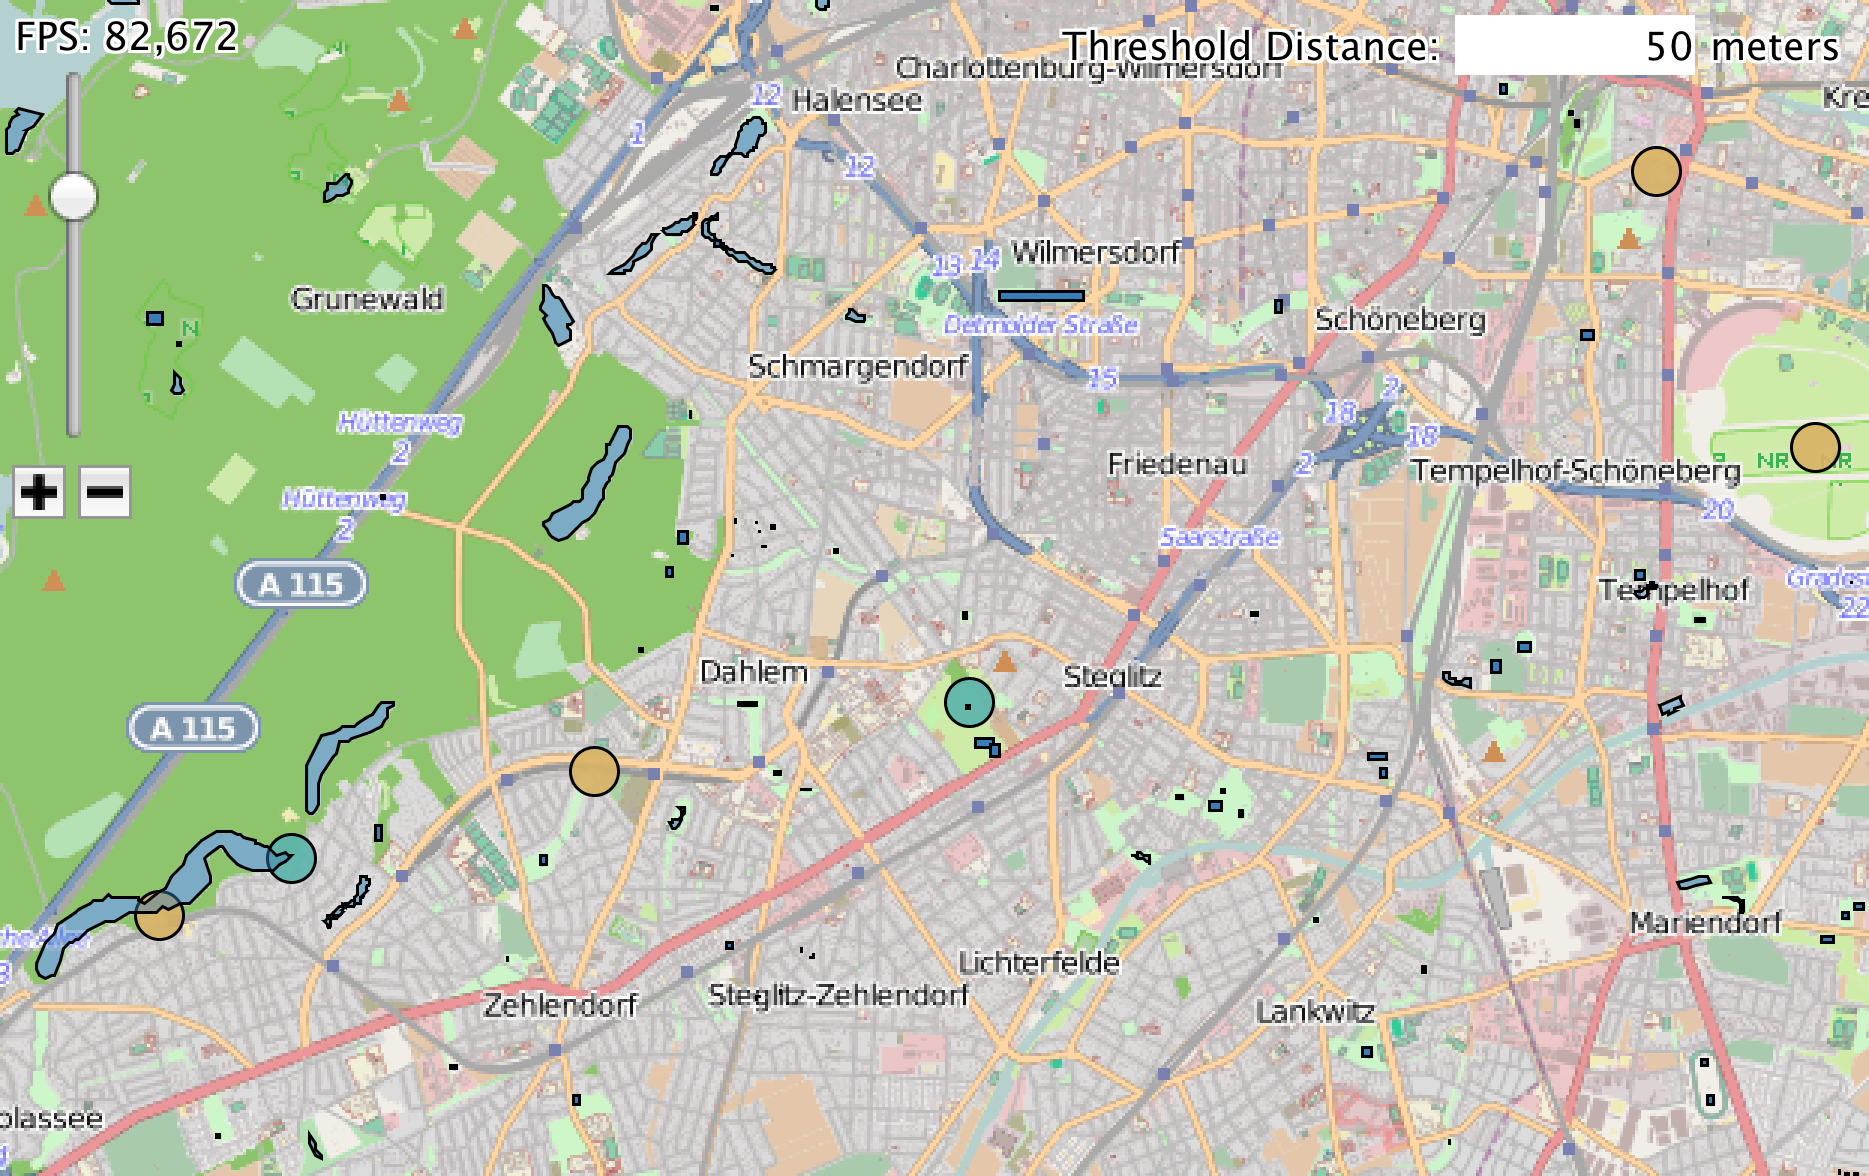
\includegraphics[width=\textwidth]{imgs/parks}
                \caption{Blue points are parks near water. Beige points represent parks further
                away from water than $50m$.}
                \label{fig:parks}
        \end{subfigure}
        \caption{Some solutions for hard tasks.}
\end{figure*}
